\documentclass[12pt]{article}

%\usepackage[T1]{fontenc}     % För svenska bokstäver
%\usepackage[swedish]{babel}  % För svensk avstavning och svenska

\usepackage{amsmath}
\usepackage{graphicx}
\usepackage{verbatim} 
\usepackage{color}
\usepackage{subfigure}
%\usepackage{hyperref} 
\usepackage{listings}

\title{Frivillig datoruppgift FAFF25}
\author{Niklas Sundin Johansson, dt08njo\\Lars Gustafson, ada10lgu }

\begin{document}
\maketitle

\section{Avbildningsfel}

\subsection{Teori}
Som Newton upptäckte så har olika våglängder av ljus olika brytningsindex i samma material, detta kallas kromatisk aberration. Fel kan uppstå även med monokromatisk ljus vid användandet av sfäriska prismor, detta kallas då sfärisk aberration. I uppgiften skall man med hjälp av, så kallad, ray tracing beräkna de fel som genereras. Genom att simulera standardstrålar och beräkna dess bana.  

Brytningslagen, $n_1 \cdot sin(\alpha _1) = n_2 \cdot sin(\alpha _2) $ används för att beräkna var fokalpunkten hamnar beroende på de två mediernas brytningsindex samt in och utfallsvinklarna vid övergången. 

Materialet BK7 används då kromatisk abberation skall beräknas. Formeln för dess brytningsindex är som nedan och gavs av uppgiften.\\
$n^2 = a_1 + a_2 \lambda^2 + a_3 \lambda^{-2}+a_4 \lambda^{-4}+a_5 \lambda^{-6}+a_6\lambda^{-8}$\\
$a_1= 2,271176$\\
$a_2 = -9.700709 \cdot 10^{-3}*\mu m^{-2}$\\
$a_3 = 0.0110971 \cdot \mu m^2$\\
$a_4 = 4.622809 \cdot 10^{-5} \cdot \mu m^4$\\
$a_5 = 1.616105 \cdot 10^{-5} \cdot \mu m^6$\\
$a_6 = -8.285043 \cdot 10^{-7} \cdot \mu m^8$

\subsection{Metod}
Först beräknas felet, som en sfärisk prism genererar när man ökar höjden,$h$, från den optiska axeln. Låt brytningindex $n_1 = 1$ och $n_2 = 1,5$ samt vara oberoende våglängd. Strålen infaller mot en konvex yta med krökningsradie $R = +0,15m$ och en diameter $D = 10cm$, samt inkommer parallelt med den optiska axeln. 
Resultaten av beräkningar plottas till en graf, figur \ref{1a} , och i den markeras även brännpunkten som fås med paraxialapproximationen, där bara strålar nära optiska axeln används $\alpha_1 = 0$.

\begin{figure}[h!]
  \centering
    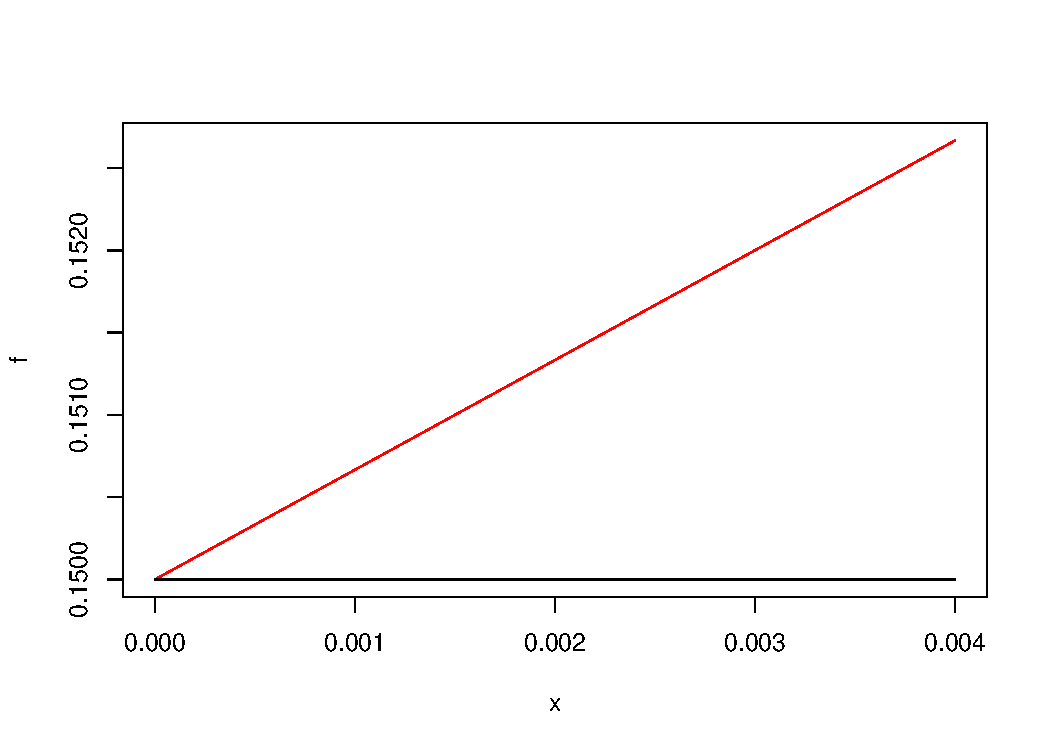
\includegraphics[scale=0.6]{para_approx.pdf}
	\caption{Illustration av sfärisk aberration.}
	\label{1a}
\end{figure} 

Nästa steg är att beräkna hur brytningsindex varierar beroende på ljusets våglängd. Genom att använda sig av funktionen som beskrevs under teoridelen för BK7 så plottas en graf där brytningsindex beräknas i intervallet $400 nm$ och $700 nm$. Grafen finns i figur \ref{1b}. 

\begin{figure}[h!]
  \centering
   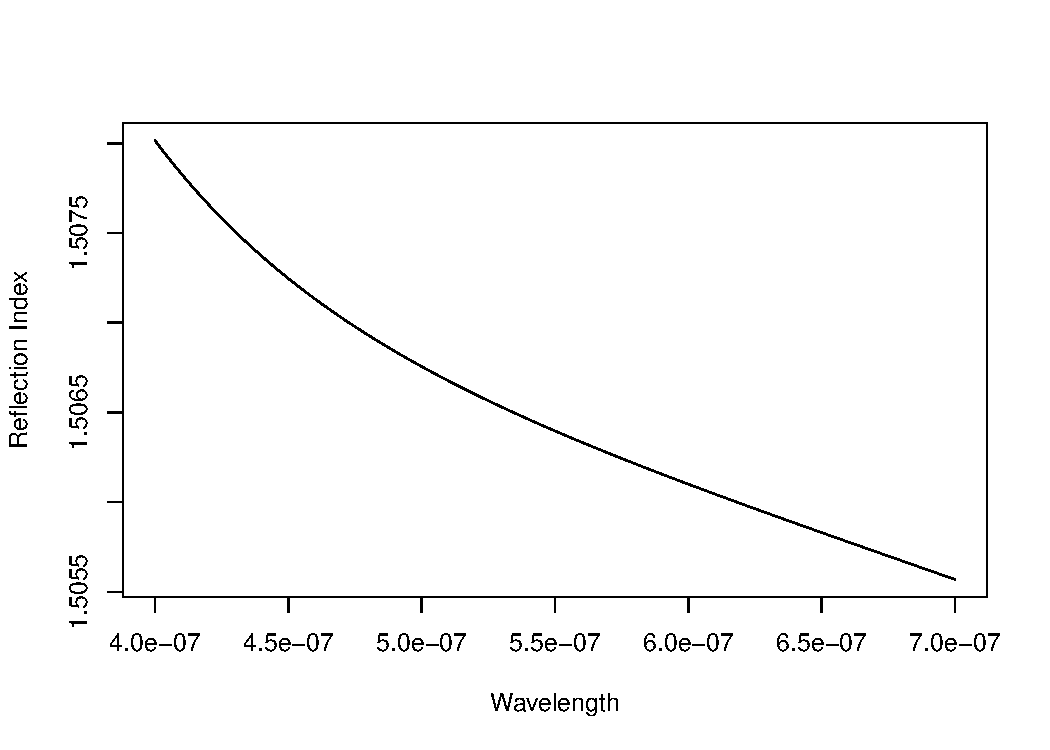
\includegraphics[scale=0.6]{BK7_index.pdf}
	\caption{Brytningsindex som en funktion av våglängd i materialet BK7.}
	\label{1b}
\end{figure} 

Slutligen skall kromatisk aberration illustreras då ljus infaller på en lins av BK7. Linsen storlek kvarstår från tidigare men brytningsindex skall beräknas för de olika våglängderna. Ljuset infaller på en höjd av $2,5 cm$ över optiska axeln. Svaret skall illustreras in en graf, figur \ref{1c}, där fokalpunkten är en funktion av våglängden.

\begin{figure}[h!]
  \centering
   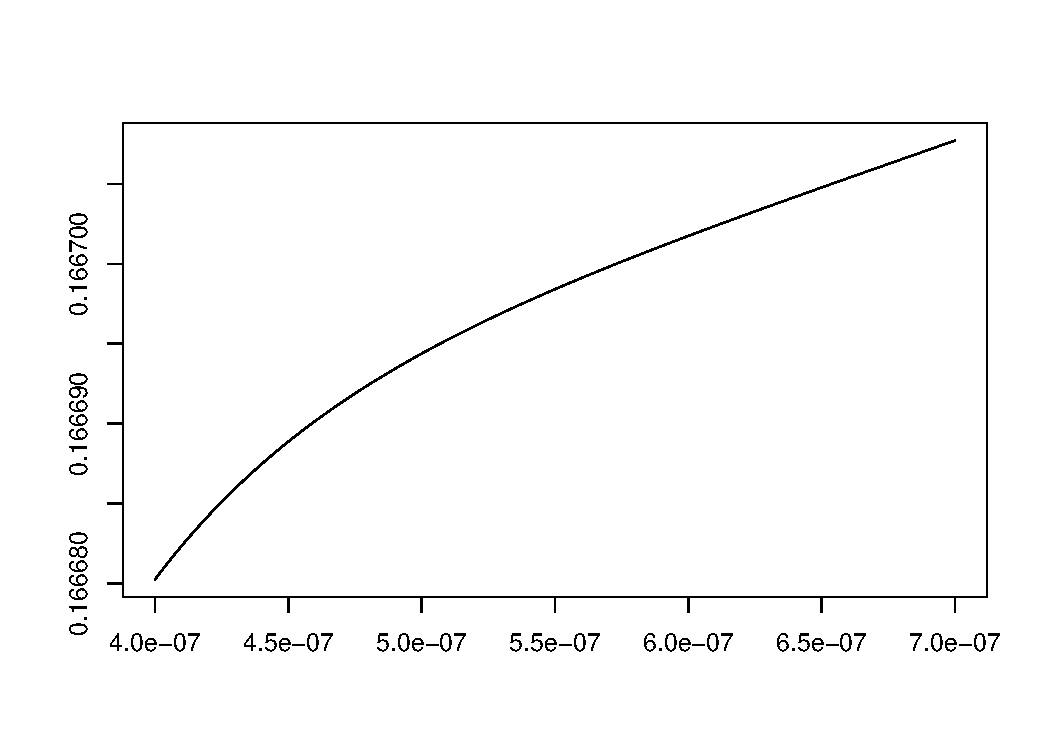
\includegraphics[scale=0.6]{BK7_abo.pdf}
	\caption{Kromatisk aberration i BK7 vid olika våglängder.}
	\label{1c}
\end{figure} 

\subsection{Resultat}
Enligt figur \ref{1a} så kan man se att fokalpunkten förskjuts med $2,6671 mm$ då ljuset infaller vid toppen av prisman istället för rakt på optiska axeln.

\noindent
Fokalpunkten i BK7 har en varians på $2,74 10^{-5}m$ vilket kan ses i figur \ref{1c}.

%går från 1.508016 till 1.505569

%går från 0.1666803 till 0.1667077

\subsection{Slutsats}
Enligt beräkningarna så är det bevisat att både kromatisk och sfärisk aberration existerar. Dock tycks det vara så att den sfäriska är betydligt större än den kromatiska. I alla fall för det material vi testat för.

\subsection{Analys}
Felen som uppstår i experimenten kan man anse är väldigt låga. Det får en att tro att approximatiner kan användas vid de flesta beräkningar och man behöver varken ta hänsyn till höjden ovanför den optiska axeln eller varierande våglängd. Dock fick vi en väldigt begränsad mängd material att testa på. Materialet BK7 sägs vara en vanlig glassort och kan därför vara ett material som är framtaget för dess bra egenskaper. Detta går inte att utröna utan djupare efterforskning i materialet samt fler tester med andra material.


\section{Pulsade lasrar}

\subsection{Teori}

\subsection{Metod}

\subsection{Resultat}

\subsection{Slutsats}

\subsection{Analys}


\subsection{Result}
\subsubsection{A: Nummeric Solution}

\subsubsection{B: Differential Plot}
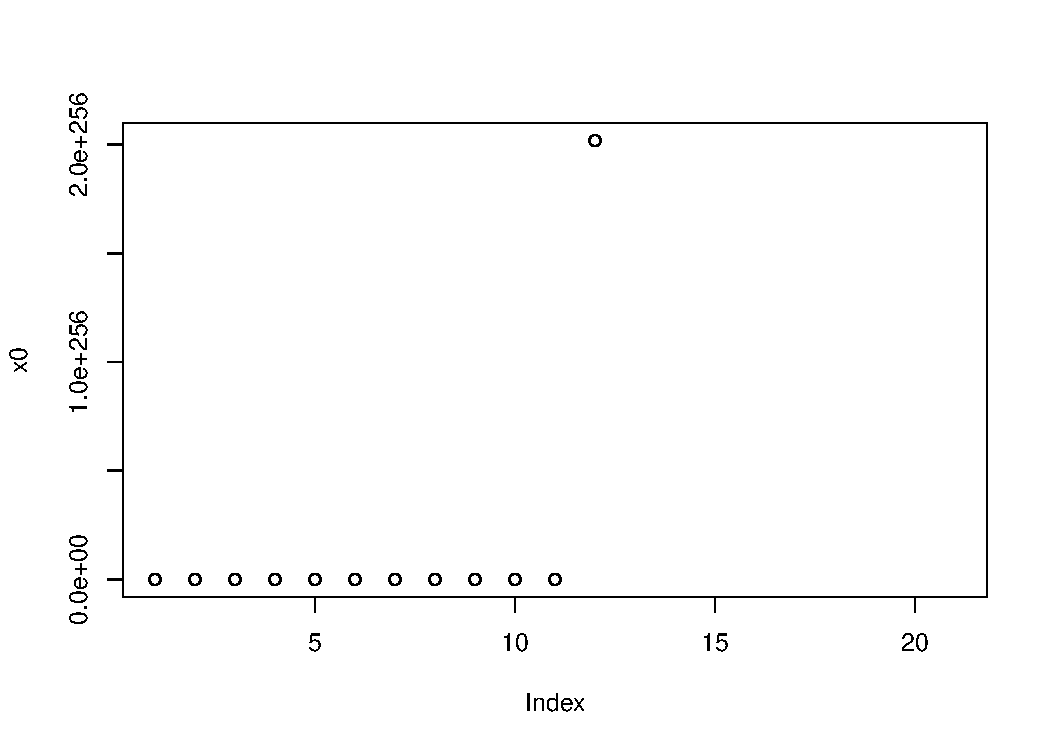
\includegraphics[scale=0.6]{N.pdf}

\subsection{Conclusion and Commentary}

\subsection{Conclusion}

\newpage
\appendix
\section{Implementation R Code}
\subsection{Assignment I:}
\lstinputlisting[numbers=left, keepspaces=true, firstline=0, lastline=68, language=R, basicstyle=\ttfamily\tiny]{datoruppgift.r}
\subsection{Assignment II: }
\lstinputlisting[numbers=left, keepspaces=true, firstline=68, basicstyle=\ttfamily\tiny]{datoruppgift.r}
\end{document}
